\begin{figure}[H]
  \centering
  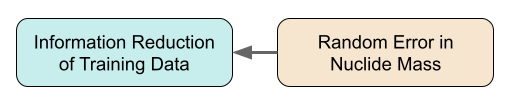
\includegraphics[width=0.7\linewidth]{./chapters/exp1/methodology1_2.png}
  \caption[Second portion of the flowchart from Figure \ref{fig:method1}]
          {Second portion of the flowchart from Figure \ref{fig:method1} being 
           described in this section.}
\end{figure}

In this section, the information quality reduction is implemented as increasing
the error of the nuclide mass measurements in the training database. After
this, the statistical models will be evaluated as to how they perform under
increasing error in the nuclide measurements. 

The training database for the first experiment is meant to be a proof of
principle with the developed methodology, and mimic a scenario where there is
"perfect knowledge" of a set of nuclides of interest.  But the overall goal of
this project is to determine how much information to what quality is needed to
train an \gls{ML} model that can provide \gls{SNF} attribution by correctly
predicting the reactor type, burnup, \gls{U235} enrichment, and time since
irradiation.  Therefore error and uncertainty were injected into the nuclide
mass measurements in the training database for the machine learning algorithms
and \gls{MLL} calculations, respectively. 

\subsection{Scikit Algorithms}

For the \textit{k}-nearest neighbor and decision tree algorithms, a uniform
error is applied randomly to each nuclide mass as follows.  For a maximum error
percentage of $E_{max}$, each nuclide mass is perturbed by a random value in the
range: $[100-E_{max},100+E_{max}]$.  This occurs for 10 error levels between
$0\% < E_{max} < 20\%$: 0, 1, 2, 5, 8, 10, 12, 15, 18, 20. Therefore the $0\%$
error case represents full knowledge of nuclide masses, and that knowledge
slowly decreases up to $20\%$. 

\subsection{Maximum Log-Likelihood Calculations}

For the \gls{MLL} calculations, a uniform uncertainty was introduced to each
nuclide mass.  The uncertainty is calculated from error propagation of Equation
\ref{eq:loglike} \cite{mll_method, mll_sensitivity}.  Thus, each nuclide is
given an uncertainty of 1, 5, 10, 15, and 20\% via:
\begin{equation}
  \sigma_{Log L}^2 = \sum_i \left( 
                            \frac{x_{i,test} - x_{i,train}}{\sigma_{i,train}^2}
                            \right)^2 
                            (\sigma_{i,train}^2 + \sigma_{i,test}^2)
  \label{eq:mllunc}
\end{equation}
where $x_{i,train}$ and $x_{i,test}$ are the nuclide measurements for the
simulated/training set samples and the test samples, respectively, and
$\sigma_{i,train}$ and $\sigma_{i,test}$ are their respective standard
deviations calculated from the four uncertainty levels listed above.  
